\documentclass{article}
\usepackage[utf8]{inputenc}
\usepackage{graphicx}

\title{CR tp-bp-archi}
\author{Chloé Dorchêne et Léo Marché}
\date{November 2022}

\usepackage{geometry}
 \geometry{
 a4paper,
 left=30mm,
 right=30mm,
 top=30mm,
 }

 \graphicspath{{courbes/}}

\begin{document}

\maketitle

\section{Prédicteurs simples}

\subsection{Prédicteur bimodal}

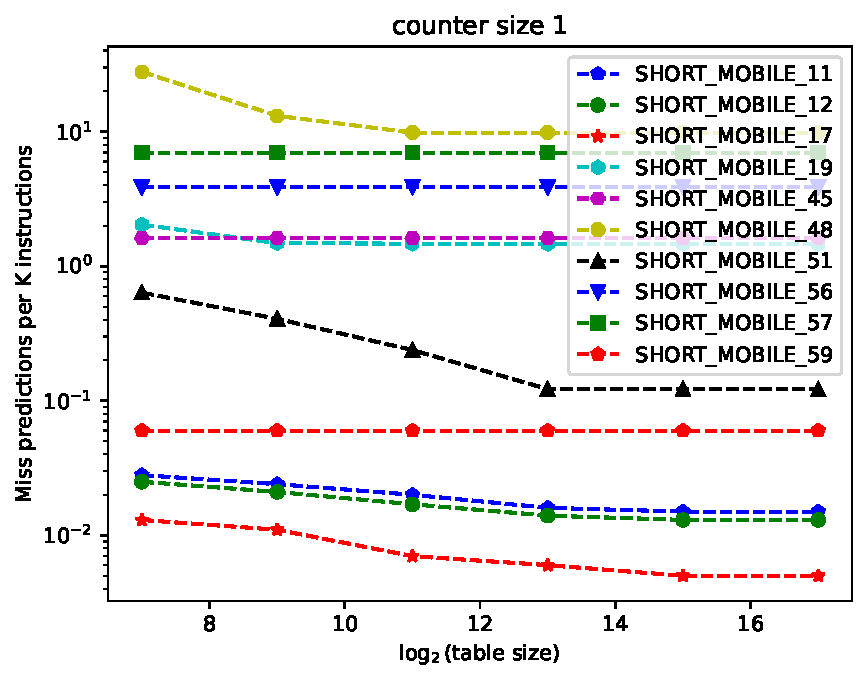
\includegraphics[width=.5\textwidth]{bimodal/graph_1.pdf}
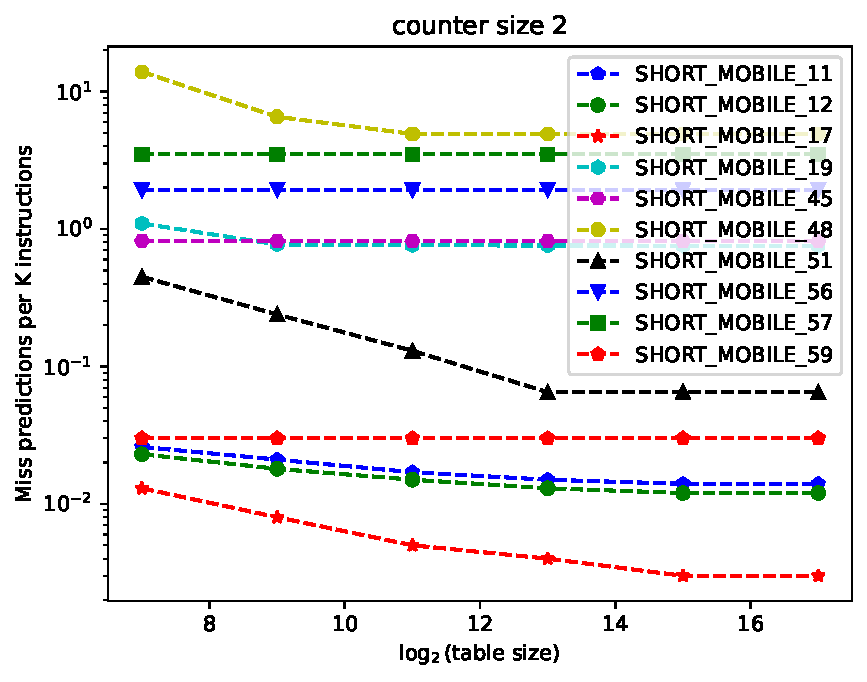
\includegraphics[width=.5\textwidth]{bimodal/graph_2.pdf}
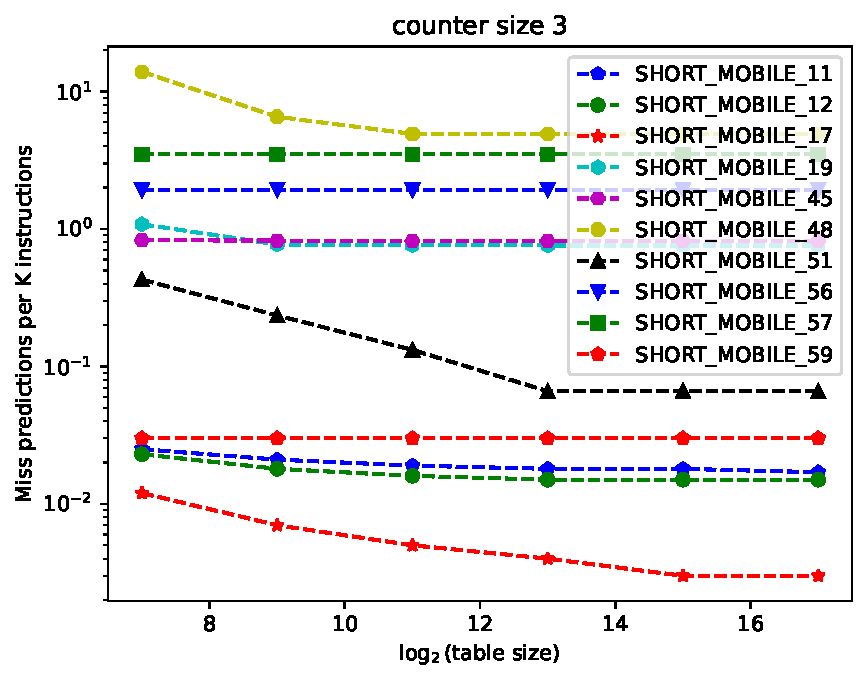
\includegraphics[width=.5\textwidth]{bimodal/graph_3.pdf}
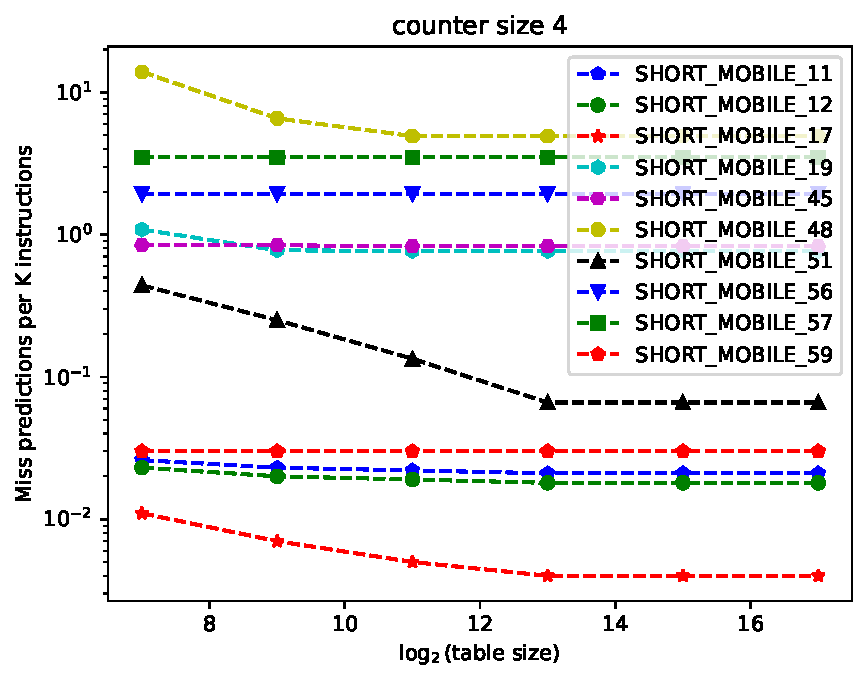
\includegraphics[width=.5\textwidth]{bimodal/graph_4.pdf}

\subsection{Prédicteur gshare}

\subsubsection{Historique sur pcbits}

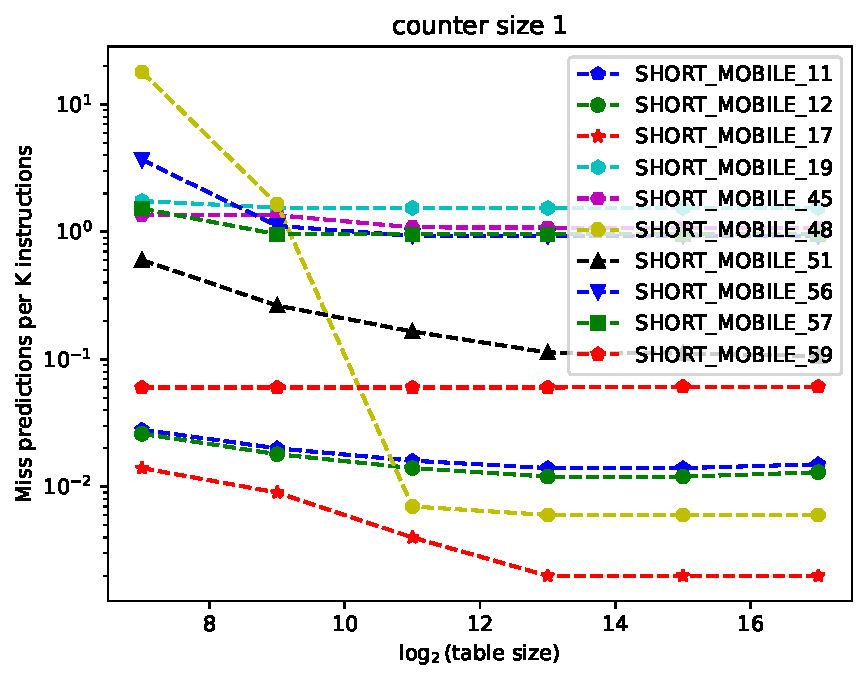
\includegraphics[width=.5\textwidth]{gshare/hmax/graph_1.pdf}
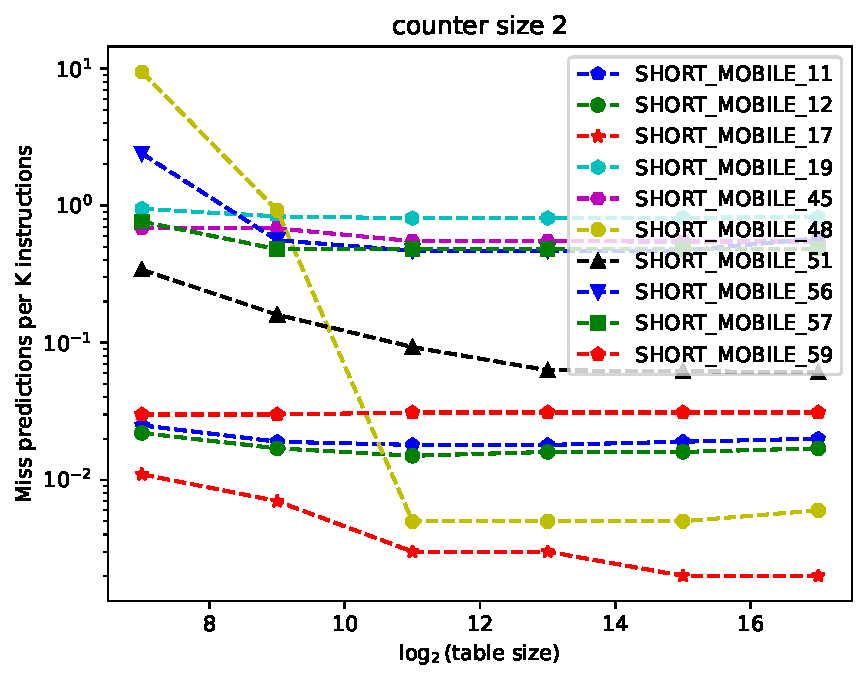
\includegraphics[width=.5\textwidth]{gshare/hmax/graph_2.pdf}
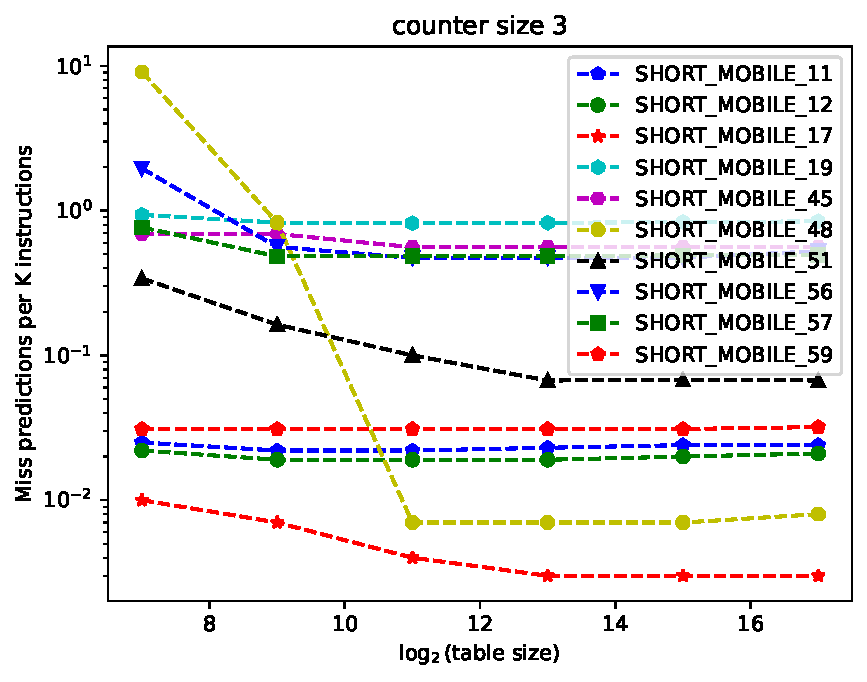
\includegraphics[width=.5\textwidth]{gshare/hmax/graph_3.pdf}
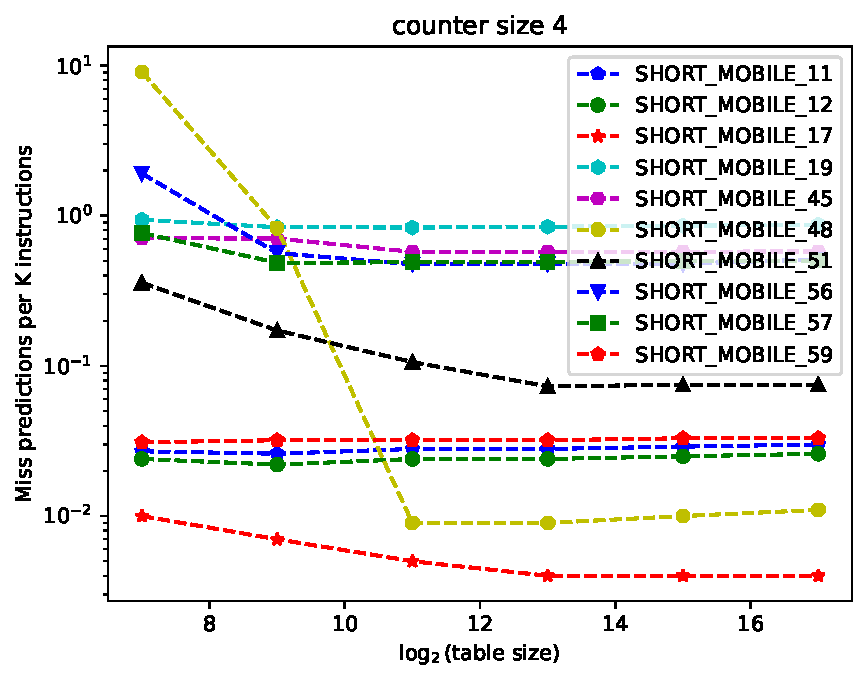
\includegraphics[width=.5\textwidth]{gshare/hmax/graph_4.pdf}

Notre première intuition avec gshare a été de nous dire que l'historique devait être au maximum sur le même nombre de bits que l'index dans la table. Nous avons donc commencés avec un masque d'historique semblable au pcmask. 

Lorsque nous avons fait varier la taille du compteur (entre 1 et 4), nous n'avons pas remarqué de réelles différences entre les prédicteurs. Certaines valeurs nous paraissent légèrement mieux sur le prédicteur avec un compteur de taille 2. Cependant, ces différences sont minimes. Les résultats restent du même ordre de grandeur quelque soit la taille du compteur. On ne peut donc pas en conclure que faire évoluer la taille du compteur influe sur la qualité des prédictions. \\

Le prédicteur gshare paraît globalement plus performant que le prédicteur bimodal. Dans l'ensemble, le prédicteur gshare aura, en ordre de grandeur, le même nombre de prédictions ratées que le prédicteur bimodal. Par contre, dans certains cas, il sera beaucoup plus performant.

Dans le cas de l'échantillon \textit{SHORT\_MOBILE\_48}, nous voyons qu'à partir d'une table de taille 2048, le prédicteur gshare est 1000 fois plus efficace. Pour des tailles de tables plus petites, il reste plus efficace même si cette différence est plus petite. 

Dans le cas inverse, le prédicteur gshare reste aussi performant que le prédicteur bimodal comme c'est le cas pour l'échantillon \textit{SHORT\_MOBILE\_19}.

\subsubsection{Historique sur 4 bits}

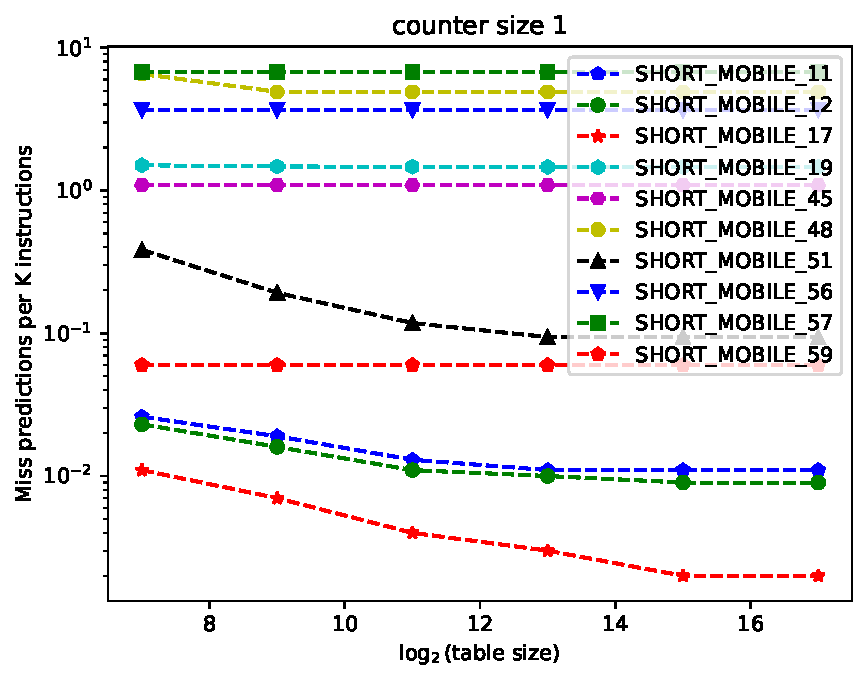
\includegraphics[width=.5\textwidth]{gshare/h4/graph_1.pdf}
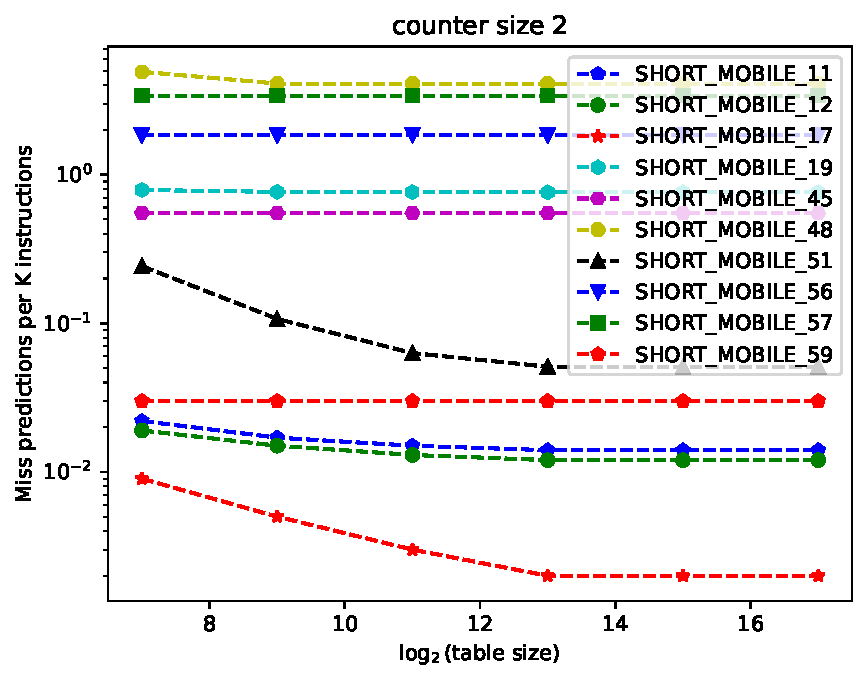
\includegraphics[width=.5\textwidth]{gshare/h4/graph_2.pdf}
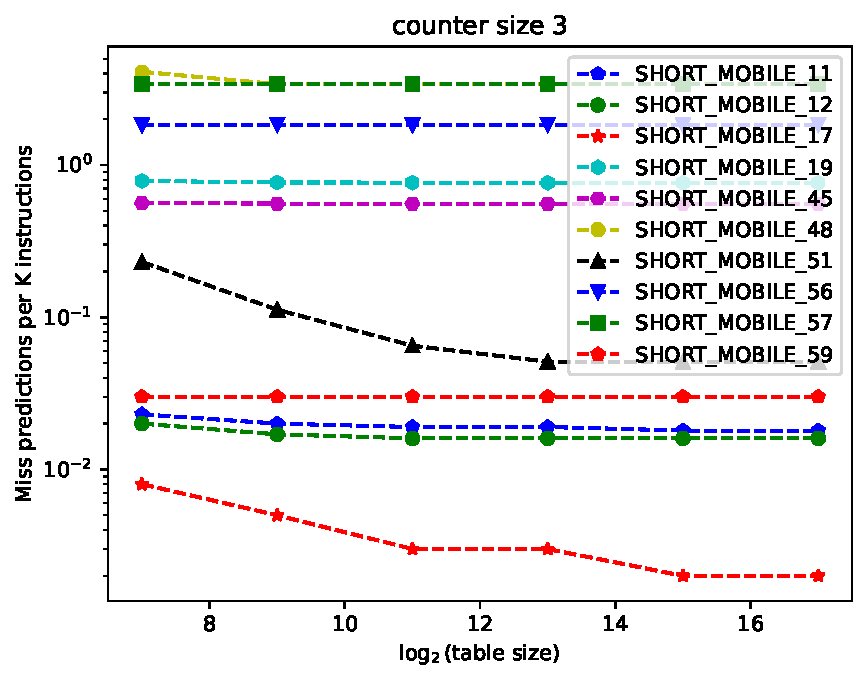
\includegraphics[width=.5\textwidth]{gshare/h4/graph_3.pdf}
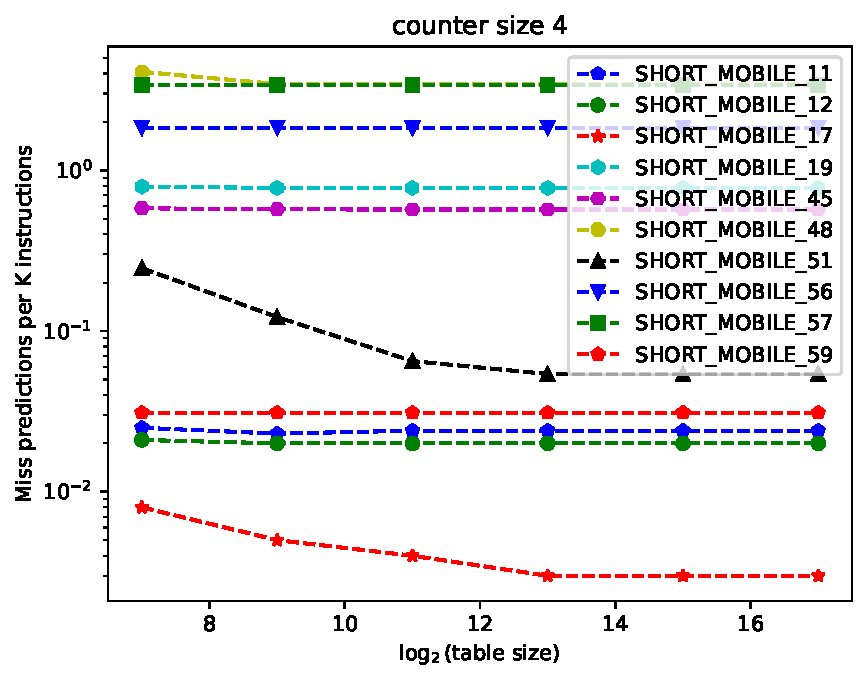
\includegraphics[width=.5\textwidth]{gshare/h4/graph_4.pdf}

Nous nous sommes ensuite dit qu'il pouvait être intéressant de réduire la taille de l'historique. Notre stratégie est d'indexer le tableau avec $(BP \oplus ((history \land historyMask) \lor (\lnot historyMask))) \land pcmask$. De cette manière, l'index est constitué du XOR entre le PC et l'historique là où c'est applicable et juste du PC là où ça ne l'est plus.

On remarque que cette stratégie est meilleure que le bimodal (même avec un historique de "seulement" 4 bits).

Nous avons choisi de tracer les courbes avec des historiques sur 4, 5 et 6 bits afin de pouvoir les comparer plus facilement avec les courbes du prédicteur local.

\subsubsection{Historique sur 5 bits}

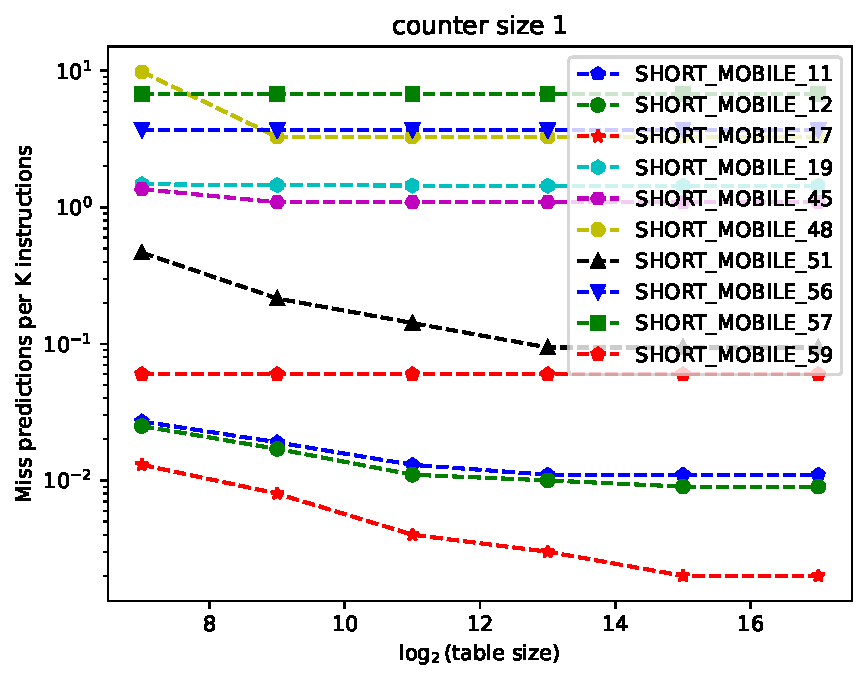
\includegraphics[width=.5\textwidth]{gshare/h5/graph_1.pdf}
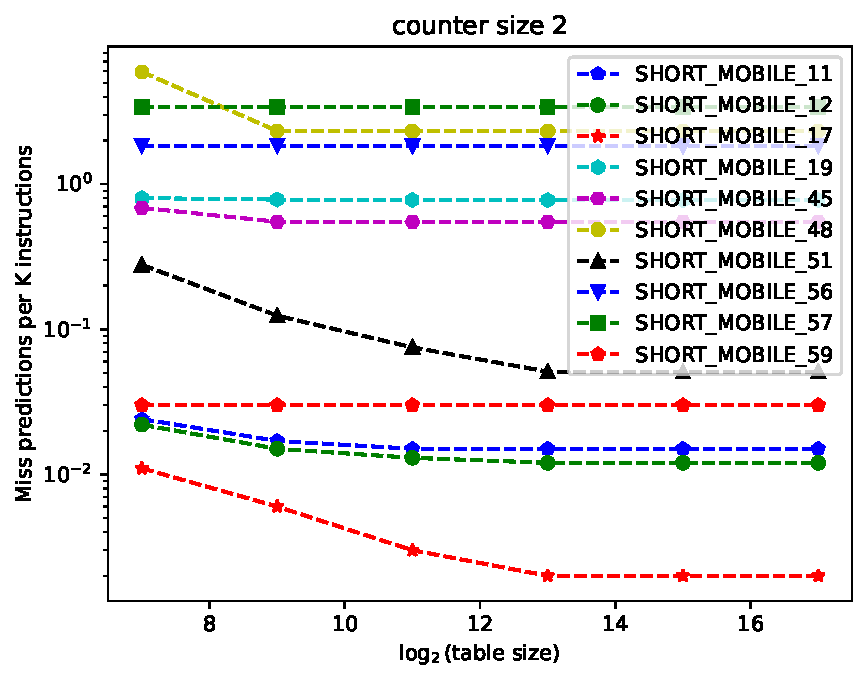
\includegraphics[width=.5\textwidth]{gshare/h5/graph_2.pdf}
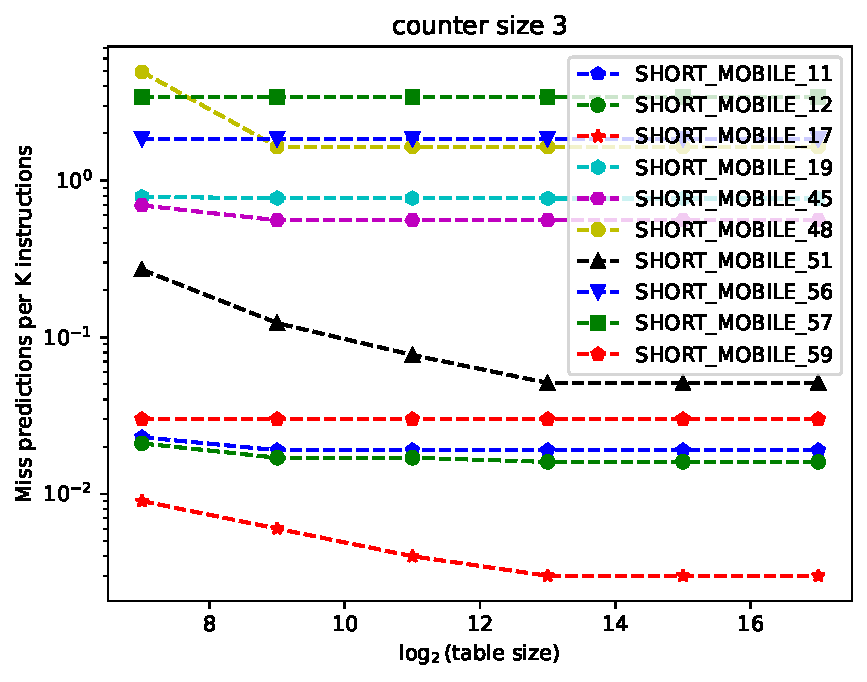
\includegraphics[width=.5\textwidth]{gshare/h5/graph_3.pdf}
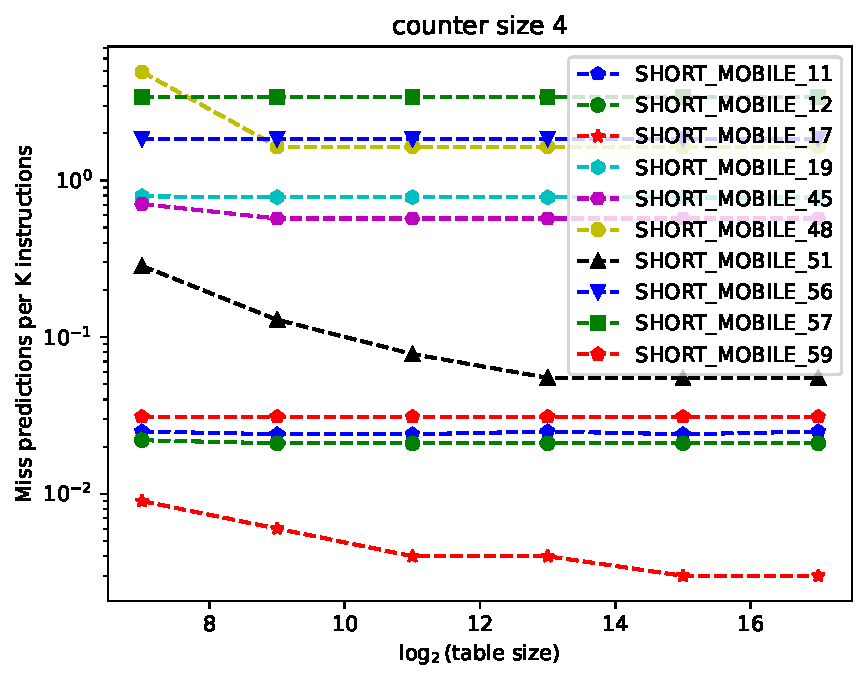
\includegraphics[width=.5\textwidth]{gshare/h5/graph_4.pdf}

L'historique sur 5 bits permet des meilleurs résultats que l'historique sur 4 bits. Cela se remarque surtout pour l'échantillon \textit{SHORT\_MOBILE\_48}. Pour une taille de table de 1024, le nombre de mauvaises prédictions par instructions est de 4 pour un historique à 5 bits et de 6 pour un historique à 4 bits. Cette différence n'est pas énorme, mais elle s'amplifie avec l'historique sur 6 bits. 

\subsubsection{Historique sur 6 bits}

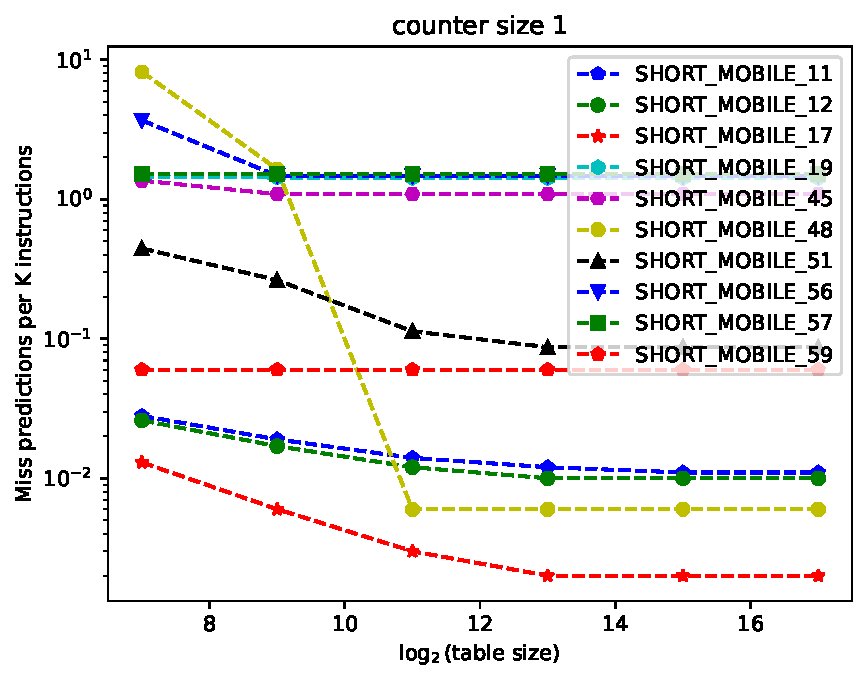
\includegraphics[width=.5\textwidth]{gshare/h6/graph_1.pdf}
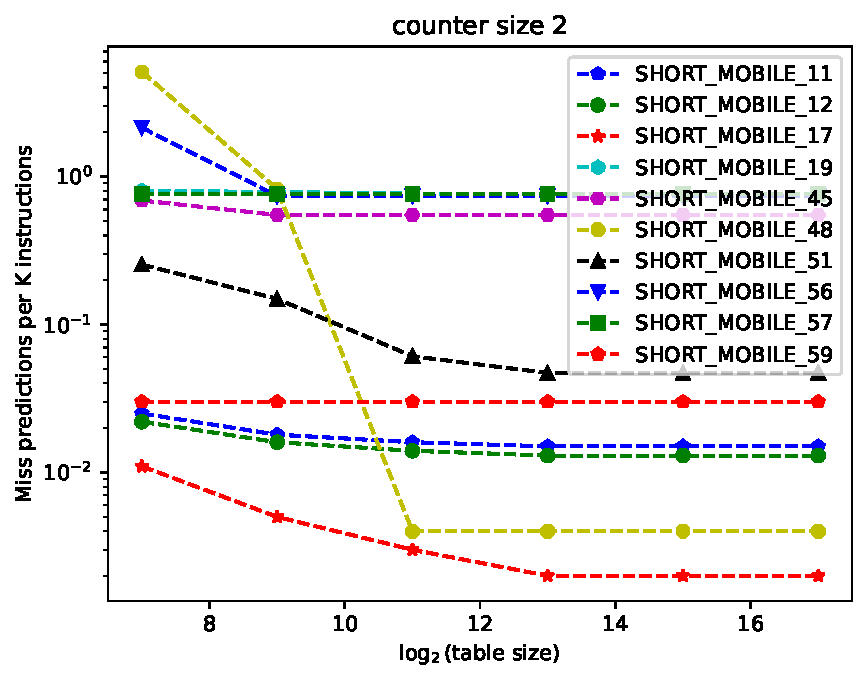
\includegraphics[width=.5\textwidth]{gshare/h6/graph_2.pdf}
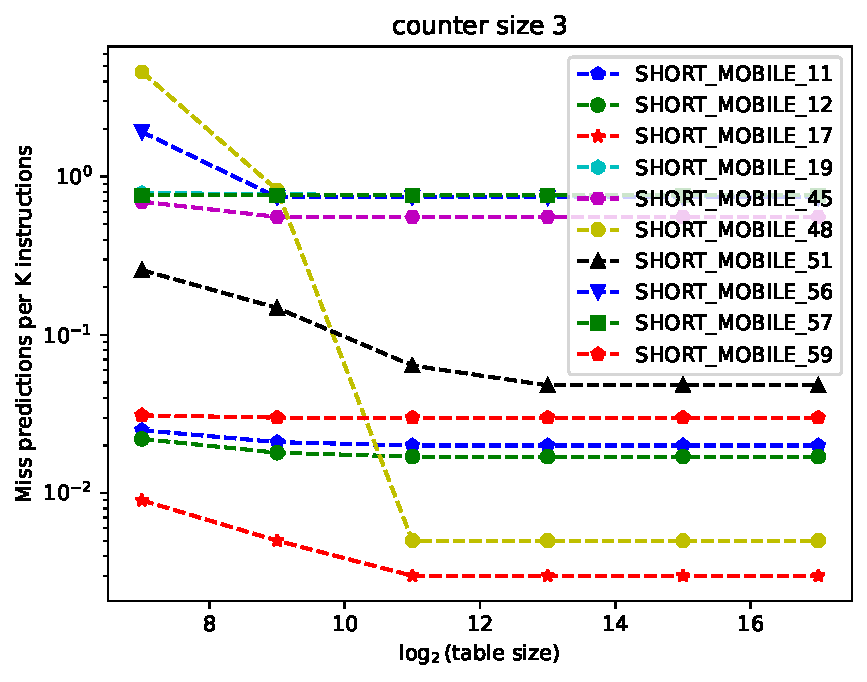
\includegraphics[width=.5\textwidth]{gshare/h6/graph_3.pdf}
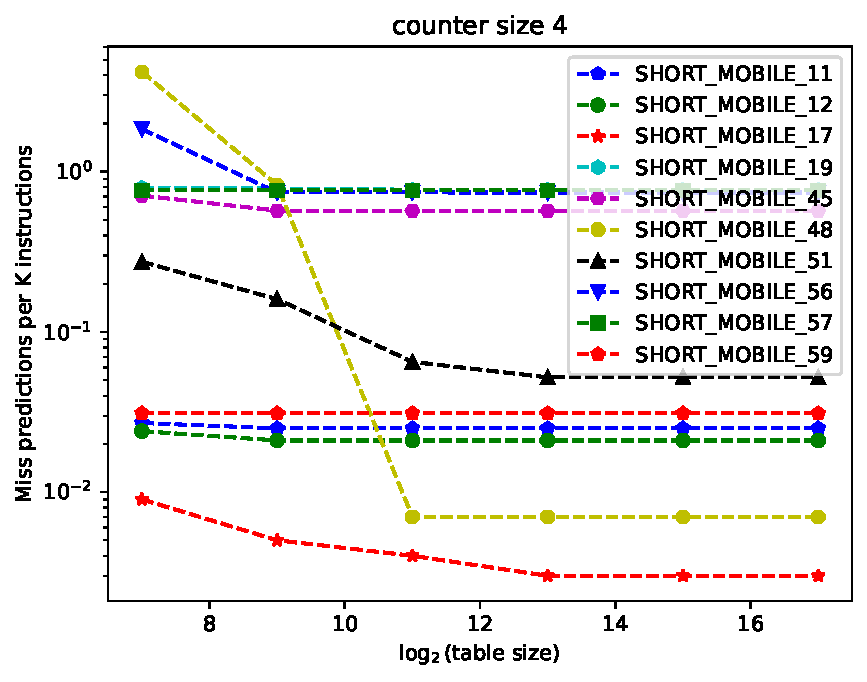
\includegraphics[width=.5\textwidth]{gshare/h6/graph_4.pdf}

C'est quand on passe à un historique sur 6 bits ou plus qu'on a les meilleures améliorations dans la prédiction de nos traces. Cela se voit particulièrement sur l'échantillon \textit{SHORT\_MOBILE\_48}. On y retrouve une amélioration comparable à celle atteinte avec un historique sur pcbits.

\subsection{Prédicteur local}

\subsubsection{Historique sur 4 bits}

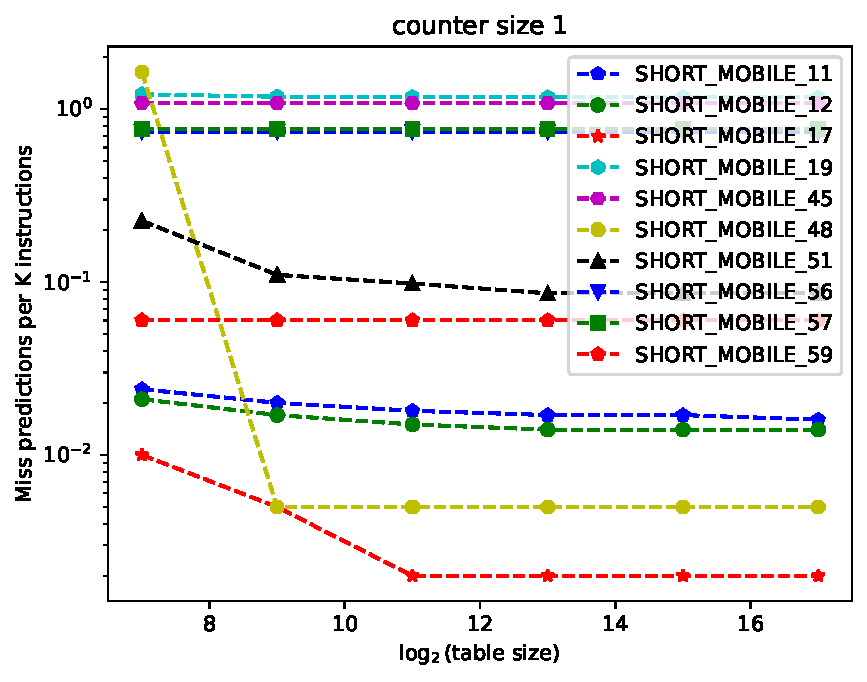
\includegraphics[width=.5\textwidth]{local/h4/graph_1.pdf}
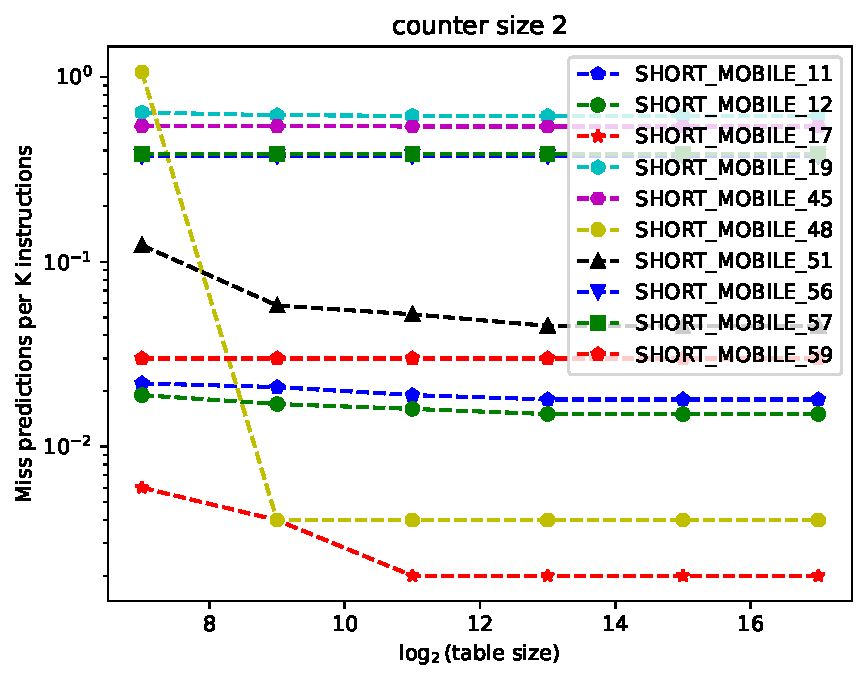
\includegraphics[width=.5\textwidth]{local/h4/graph_2.pdf}
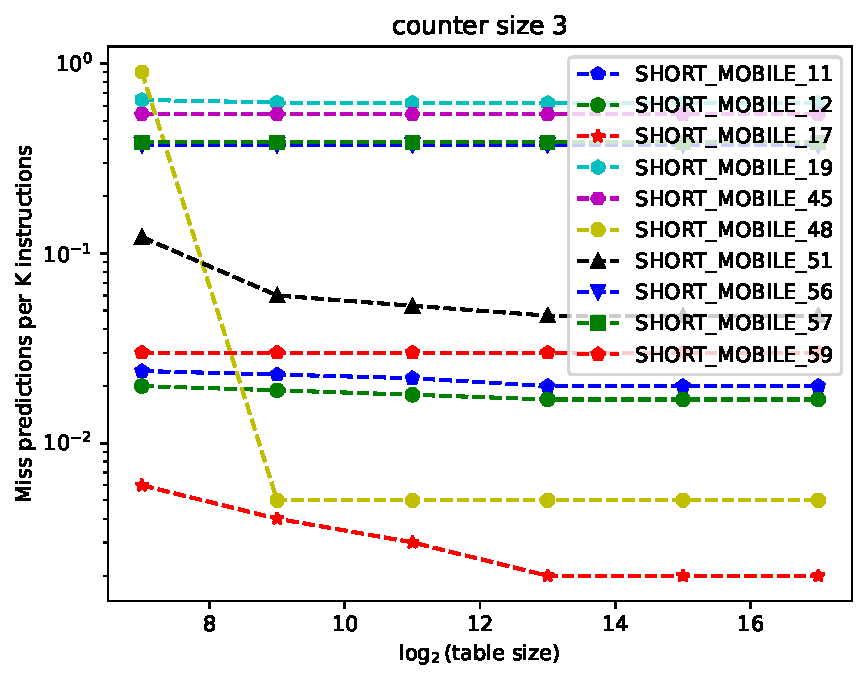
\includegraphics[width=.5\textwidth]{local/h4/graph_3.pdf}
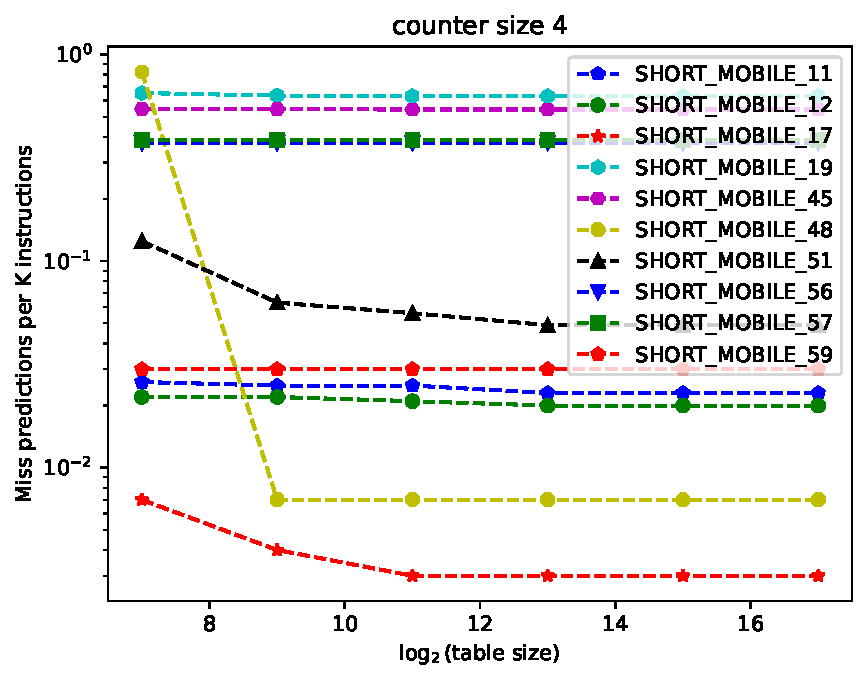
\includegraphics[width=.5\textwidth]{local/h4/graph_4.pdf}

Quel que soit le nombre de bits de l'historique pour un prédicteur gshare, le prédicteur local permet de meilleurs résultats pour les petites tailles de table, c'est-à-dire inférieur à 1024. Sur l'échantillon \textit{SHORT\_MOBILE\_48}, ce prédicteur local, avec compteur de taille 1, permet d'avoir $5.10^{-2}$ mauvaises prédictions par instructions à la place d'un pour le prédicteur gshare sur 6 bits (celui qui donne la meilleure valeur pour un compteur de taille 1).

Pour les grandes valeurs de table, il n'y a pas de grande différence entre le prédicteur gshare et le prédicteur local.

\subsubsection{Historique sur 5 bits}

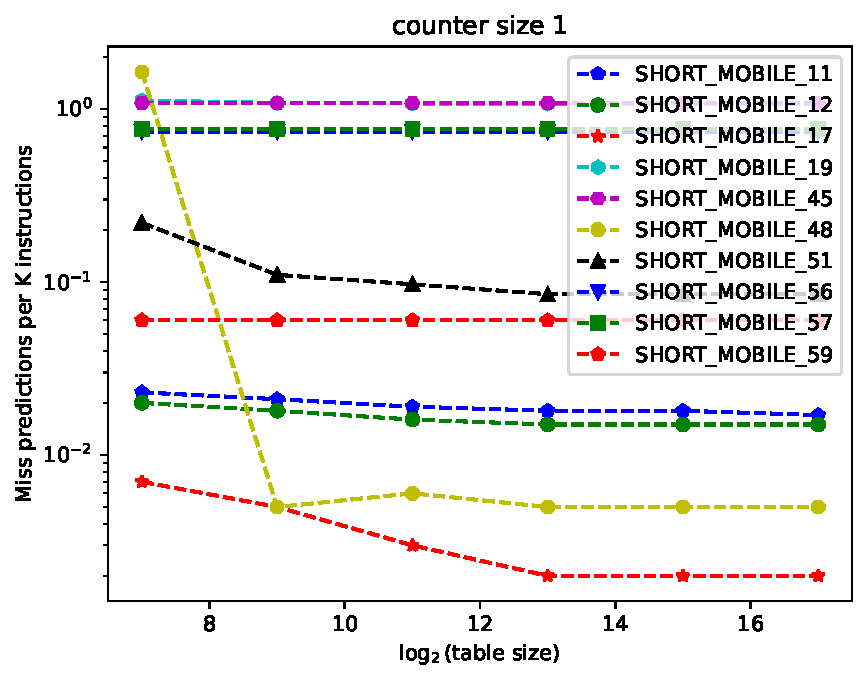
\includegraphics[width=.5\textwidth]{local/h5/graph_1.pdf}
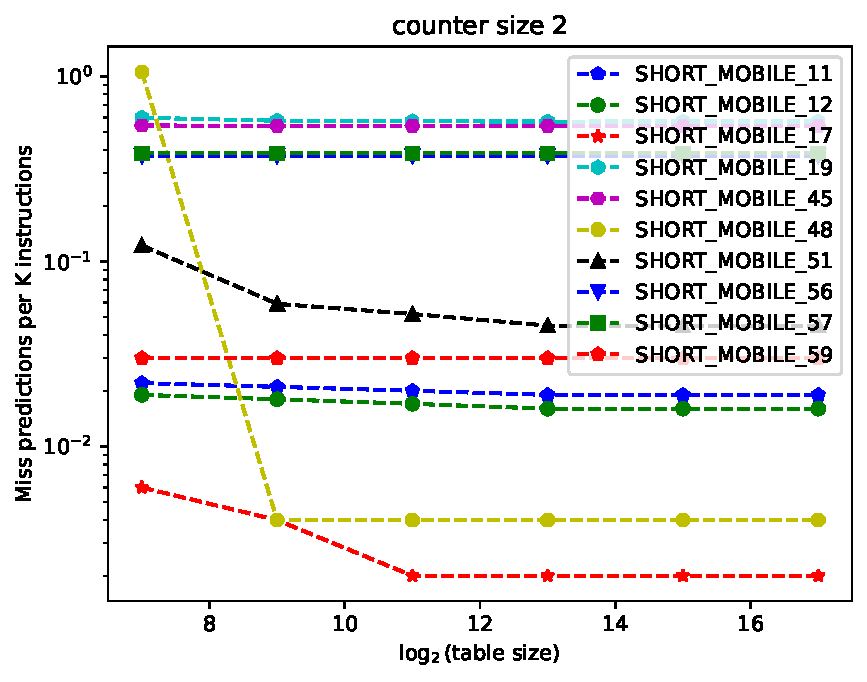
\includegraphics[width=.5\textwidth]{local/h5/graph_2.pdf}
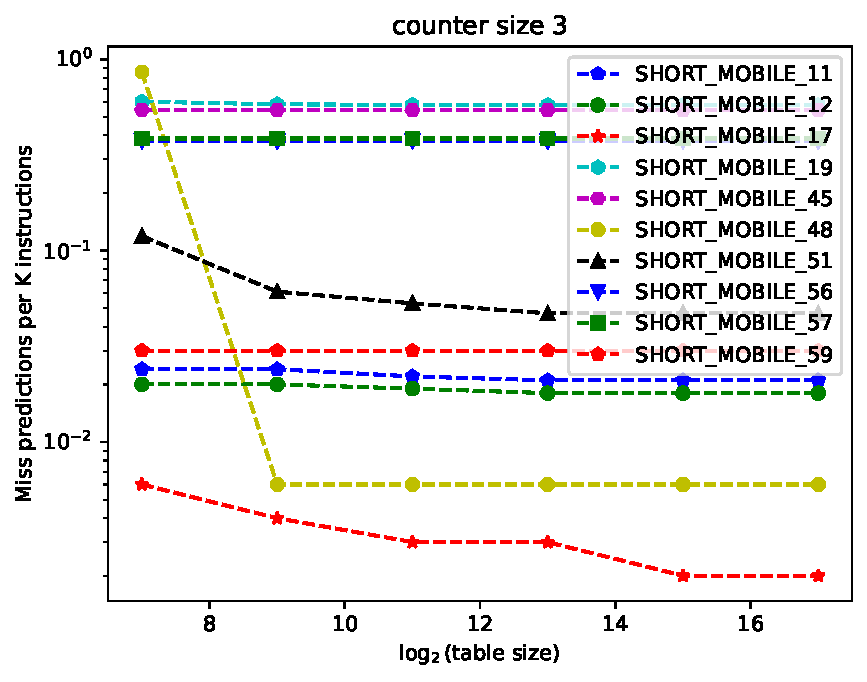
\includegraphics[width=.5\textwidth]{local/h5/graph_3.pdf}
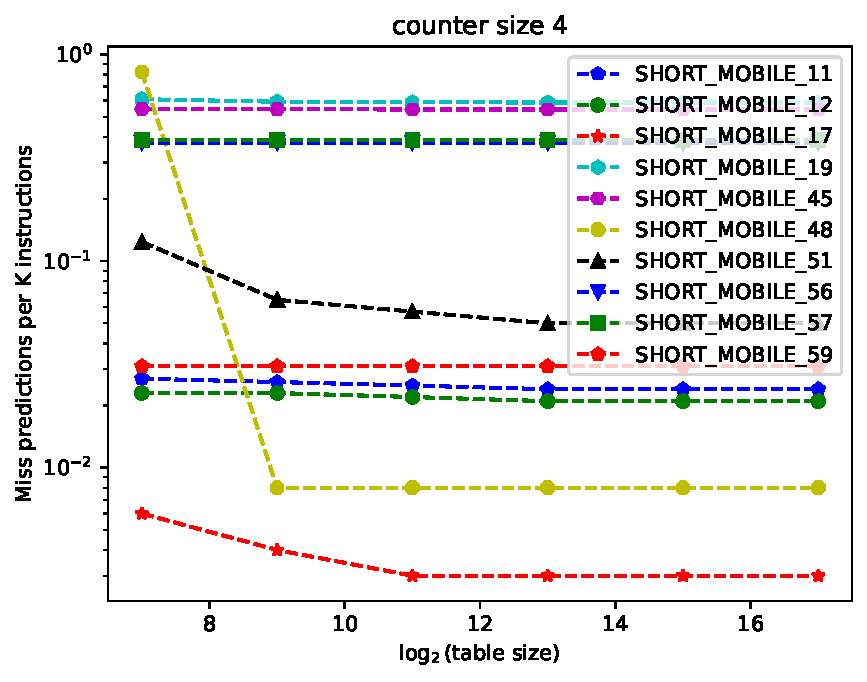
\includegraphics[width=.5\textwidth]{local/h5/graph_4.pdf}

Les valeurs obtenues pour un prédicteur local avec un historique sur 5 bits sont similaires à celles obtenues pour un prédicteur local avec historique sur 4 bits.

\subsubsection{Historique sur 6 bits}

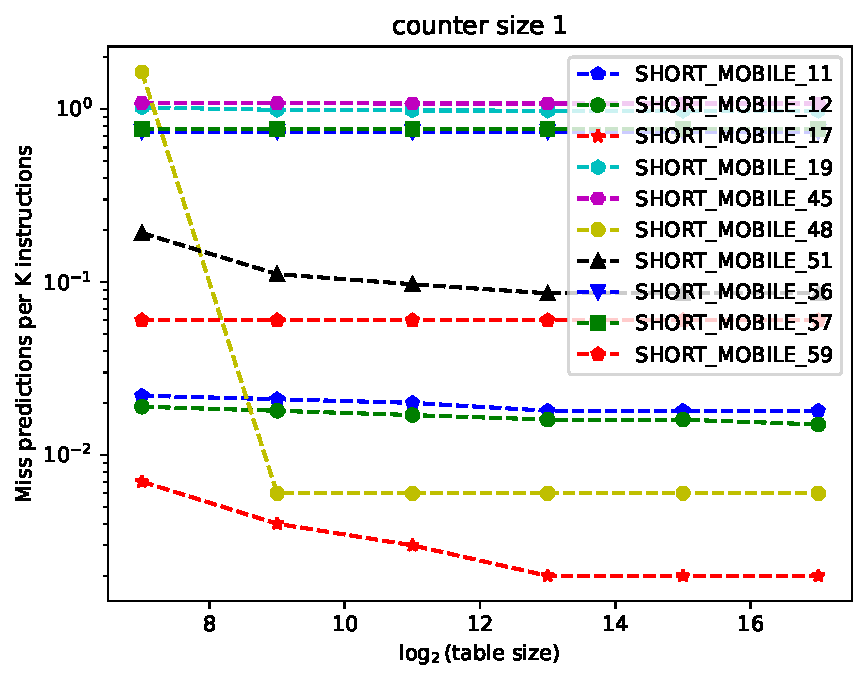
\includegraphics[width=.5\textwidth]{local/h6/graph_1.pdf}
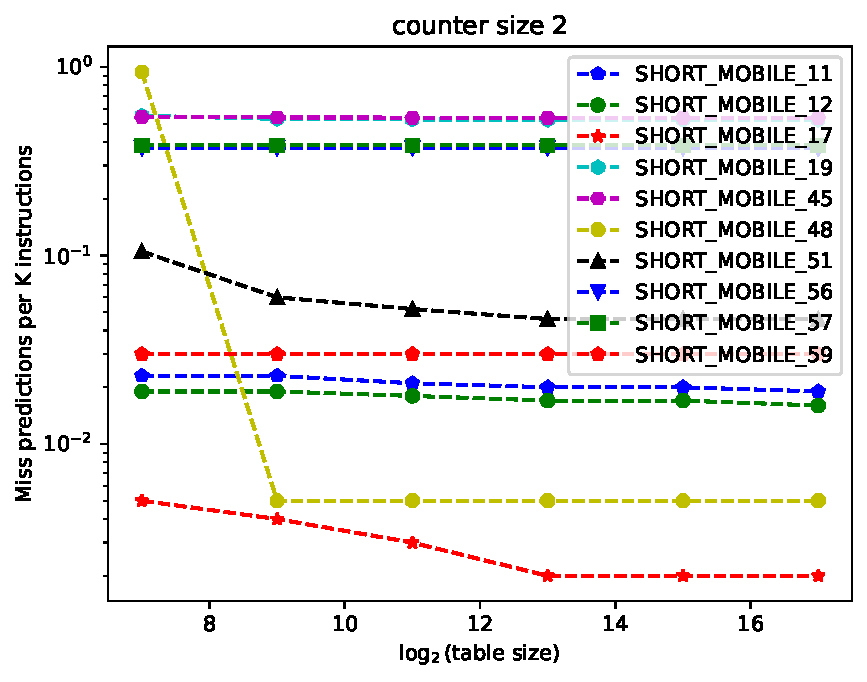
\includegraphics[width=.5\textwidth]{local/h6/graph_2.pdf}
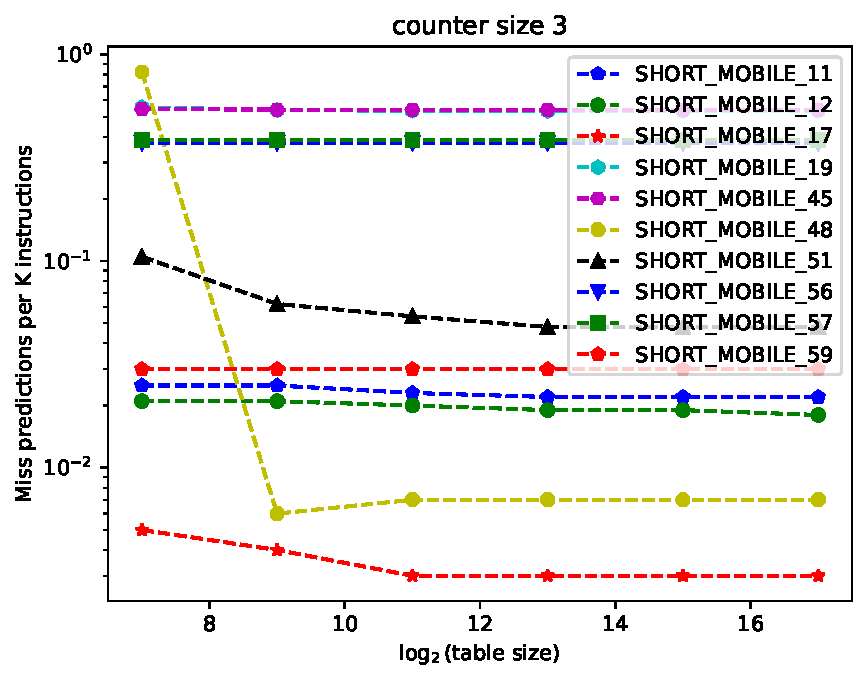
\includegraphics[width=.5\textwidth]{local/h6/graph_3.pdf}
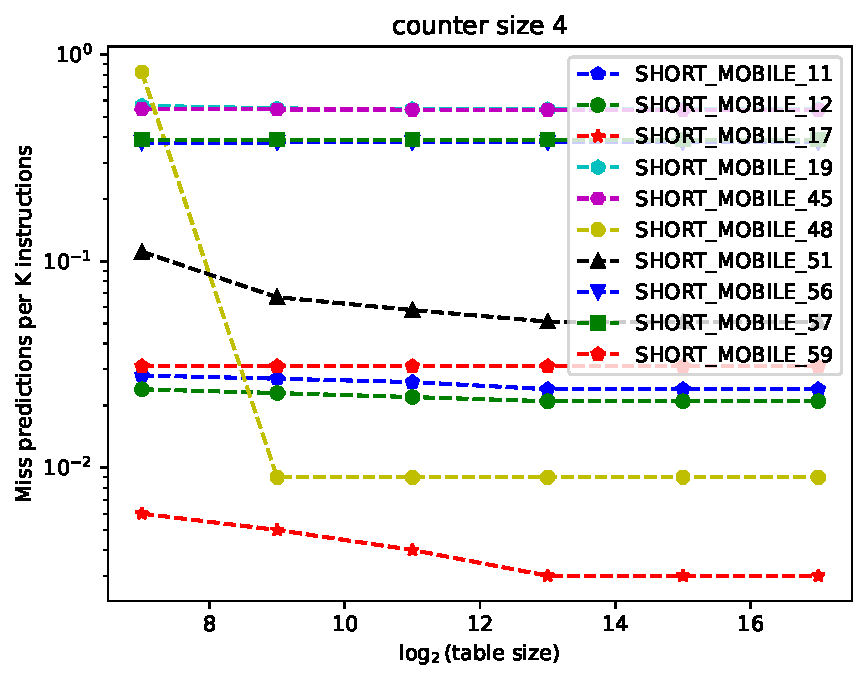
\includegraphics[width=.5\textwidth]{local/h6/graph_4.pdf}

Pour le prédicteur local avec un historique sur 6 bits, la variation de la taille de compteur n'influe pas beaucoup. La grande différence entre les graphiques est sur celui de taille de compteur valant un. Le nombre d'erreurs est plus important que pour les autres, qui à part une ou deux valeurs ont des valeurs quasi-identiques. \\

Le prédicteur local paraît plus performant que le prédicteur gshare. Le nombre d'erreurs dans les prédictions est plus petit avec le prédicteur local. Cependant, on ne retrouve pas la différence d'ordre de grandeur que nous avions trouvé entre le prédicteur gshare et le prédicteur bimodal. 

\subsection{Méta prédicteur}

\subsubsection{Historique sur 4 bits}

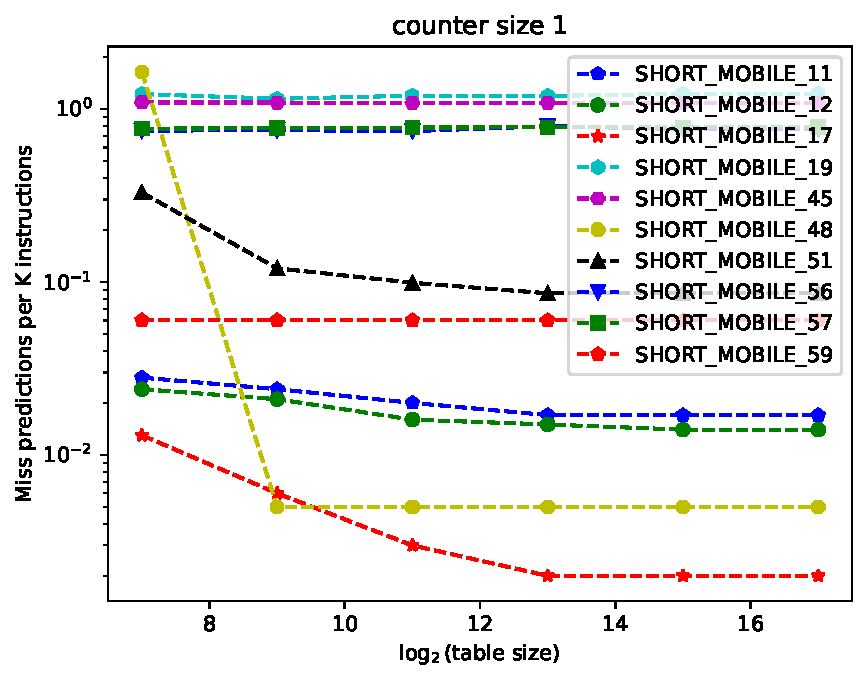
\includegraphics[width=.5\textwidth]{meta/h4/graph_1.pdf}
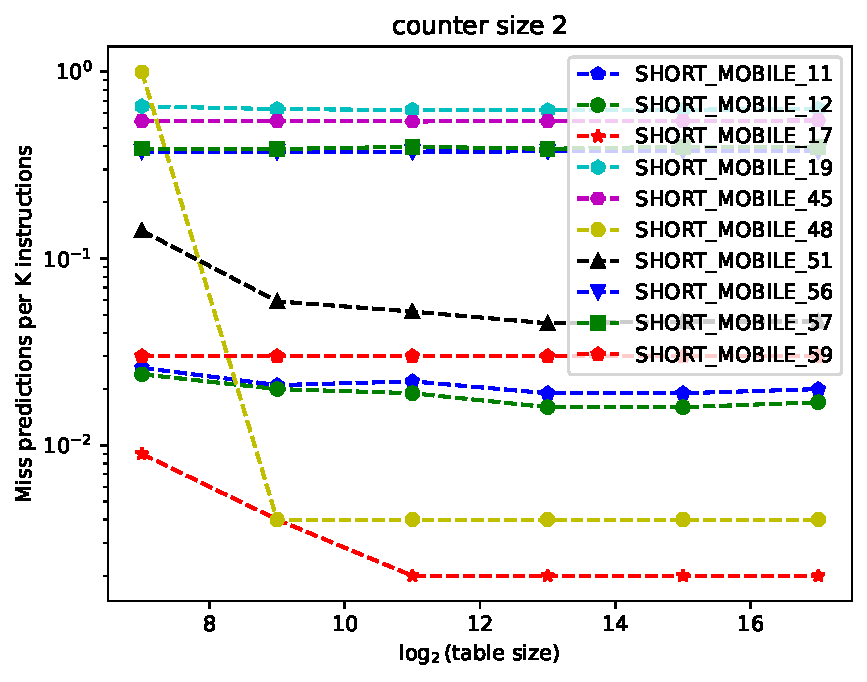
\includegraphics[width=.5\textwidth]{meta/h4/graph_2.pdf}
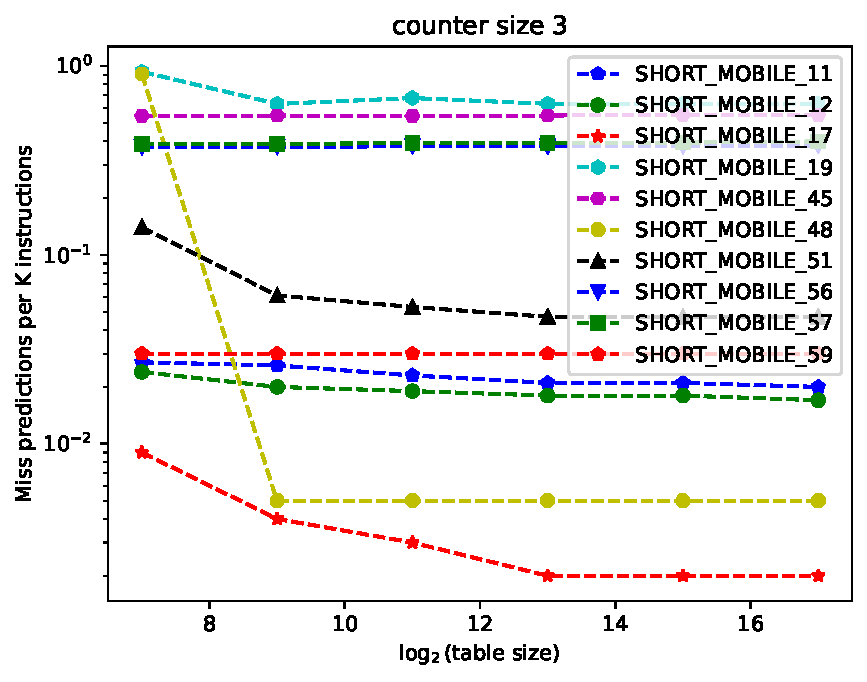
\includegraphics[width=.5\textwidth]{meta/h4/graph_3.pdf}
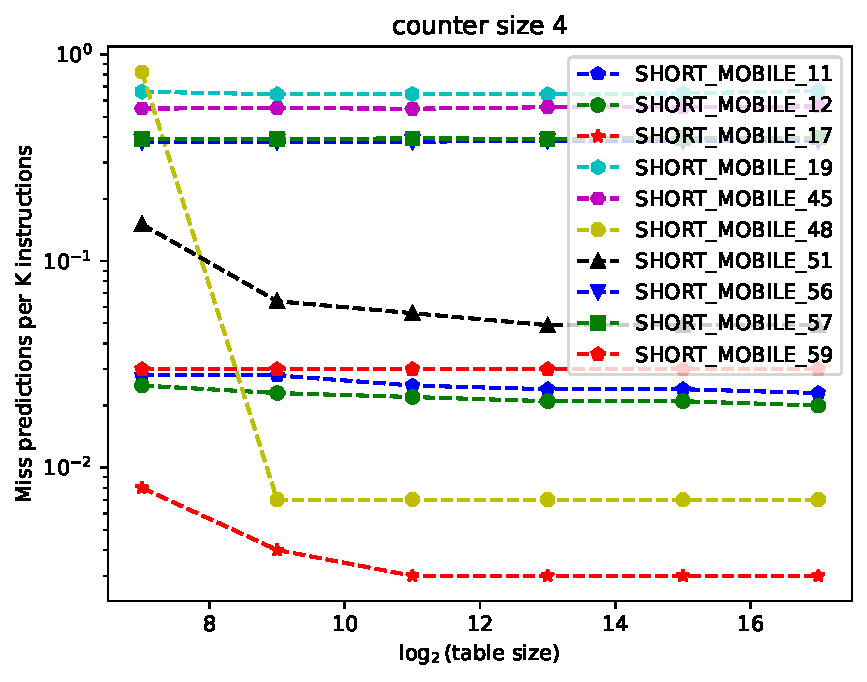
\includegraphics[width=.5\textwidth]{meta/h4/graph_4.pdf}

Quand on regarde les performances du méta prédicteur, on remarque immanquablement sa similarité avec le prédicteur local. Il semblerait que de manière générale, sur nos traces, le prédicteur local soit presque systématiquement meilleur que le gshare et que les deux prédicteur aient donc des performances assez similaires. Toutefois, on remarque quand même ces quelques petites différences:
\begin{itemize}
    \item Quand la table est petite le méta prédicteur est moins bon que le prédicteur local, probablement à cause de l'inertie ajoutée par les changements de prédicteur dans le méta prédicteur.
    \item De manière générale, le méta prédicteur est très légèrement meilleur que le prédicteur local avec de grandes tailles de tables (notamment sur la trace \textit{SHORT\_MOBILE\_48}).
\end{itemize}

\subsubsection{Historique sur 5 bits}

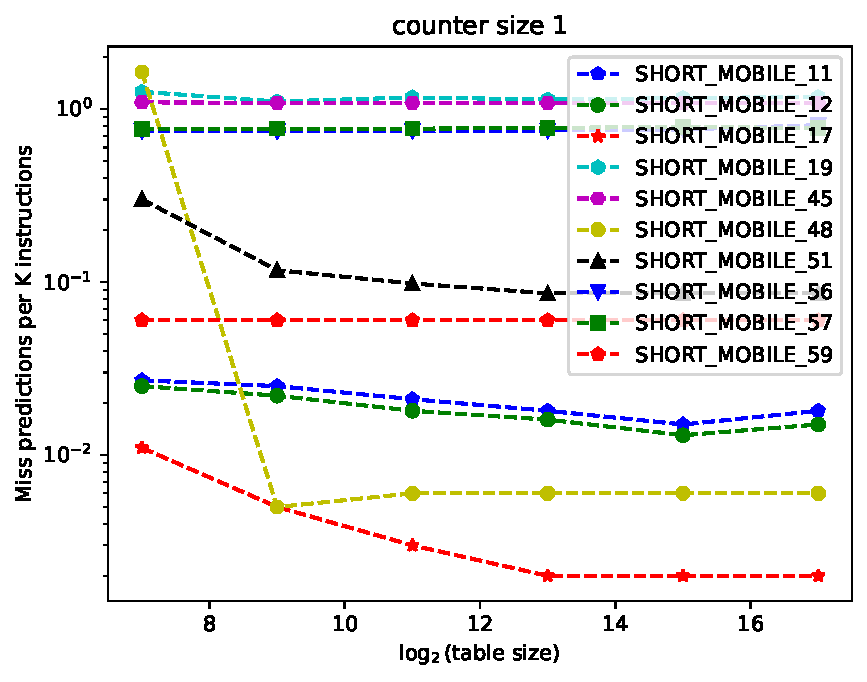
\includegraphics[width=.5\textwidth]{meta/h5/graph_1.pdf}
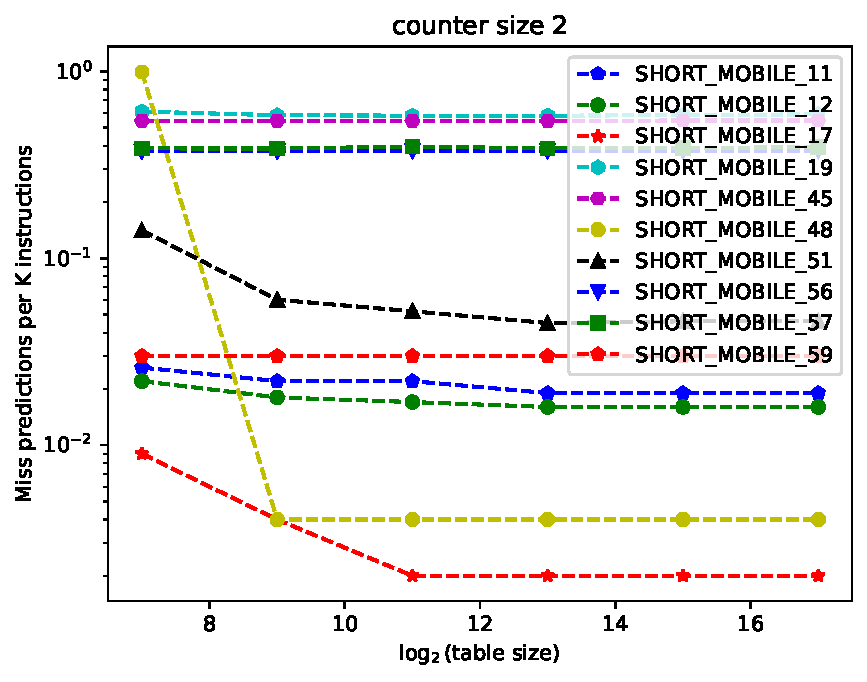
\includegraphics[width=.5\textwidth]{meta/h5/graph_2.pdf}
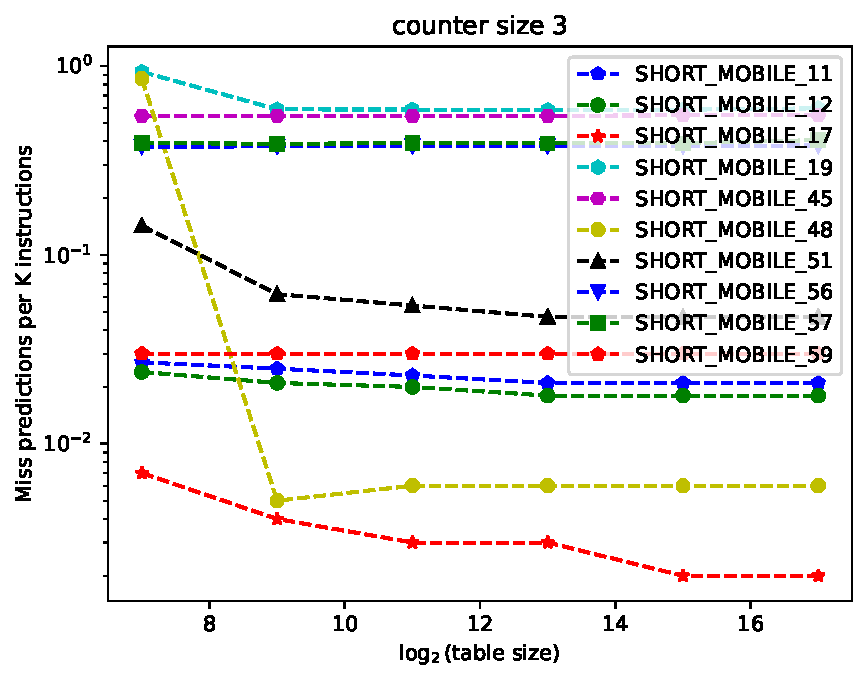
\includegraphics[width=.5\textwidth]{meta/h5/graph_3.pdf}
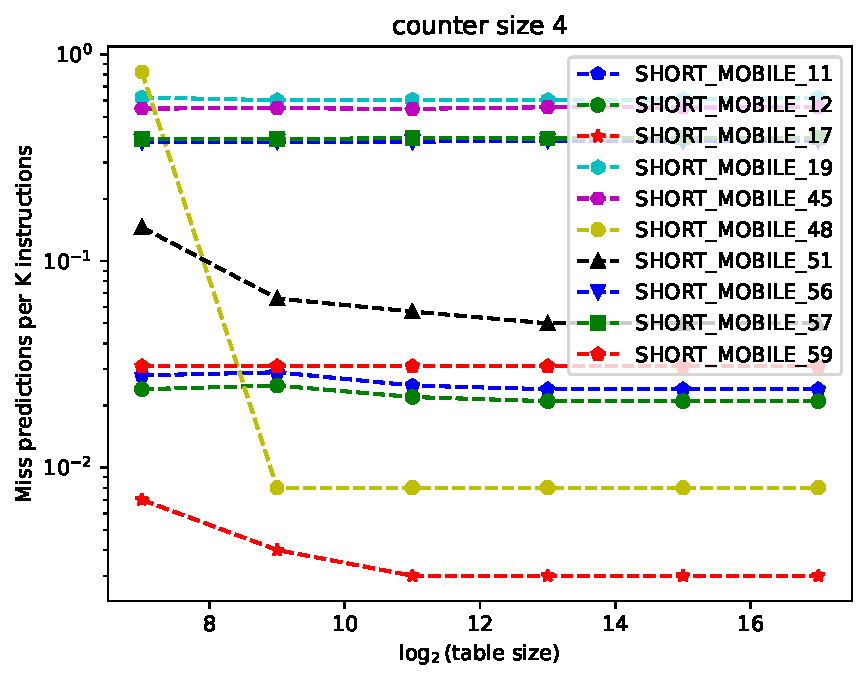
\includegraphics[width=.5\textwidth]{meta/h5/graph_4.pdf}

On fait la même remarque qu'avec un historique à 4 bits.

\subsubsection{Historique sur 6 bits}

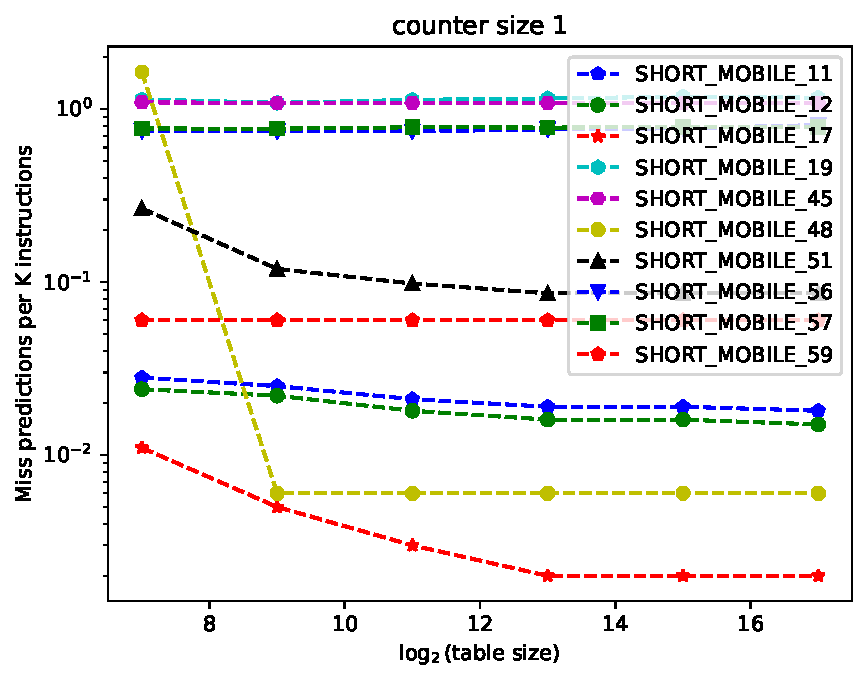
\includegraphics[width=.5\textwidth]{meta/h6/graph_1.pdf}
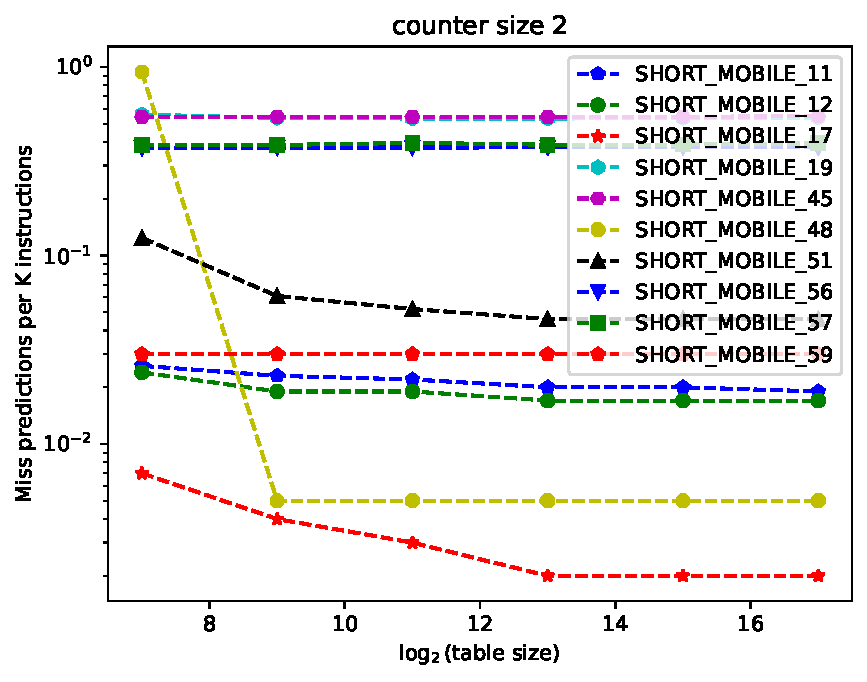
\includegraphics[width=.5\textwidth]{meta/h6/graph_2.pdf}
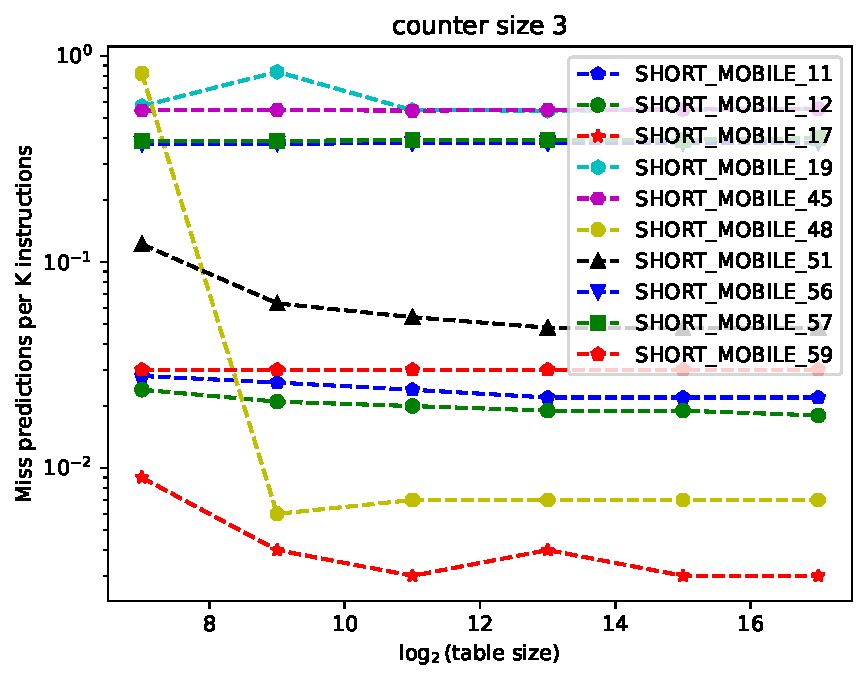
\includegraphics[width=.5\textwidth]{meta/h6/graph_3.pdf}
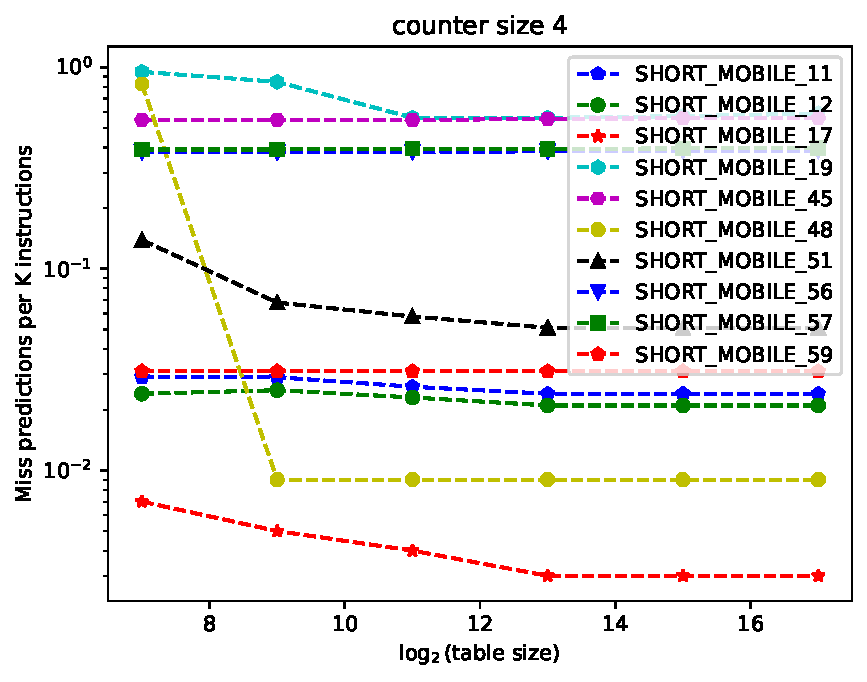
\includegraphics[width=.5\textwidth]{meta/h6/graph_4.pdf}

Sur un historique à 6 bits, on observe que le méta prédicteur est très légèrement moins bon que le prédicteur local. Cette différence n'est toutefois pas significative.

\section{Perceptron}

\subsubsection{Historique sur 4 bits}

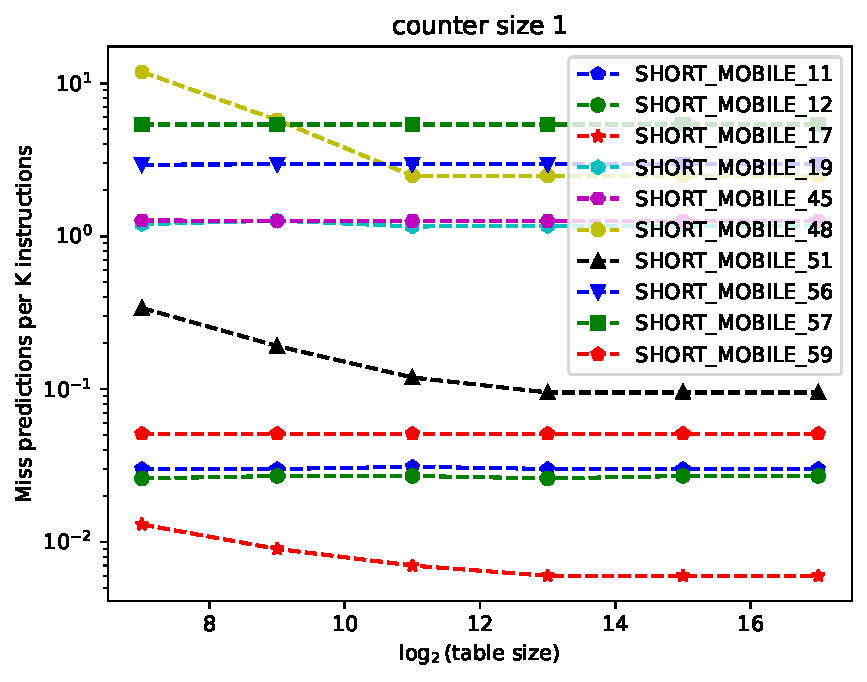
\includegraphics[width=.5\textwidth]{perceptron/h4/graph_1.pdf}
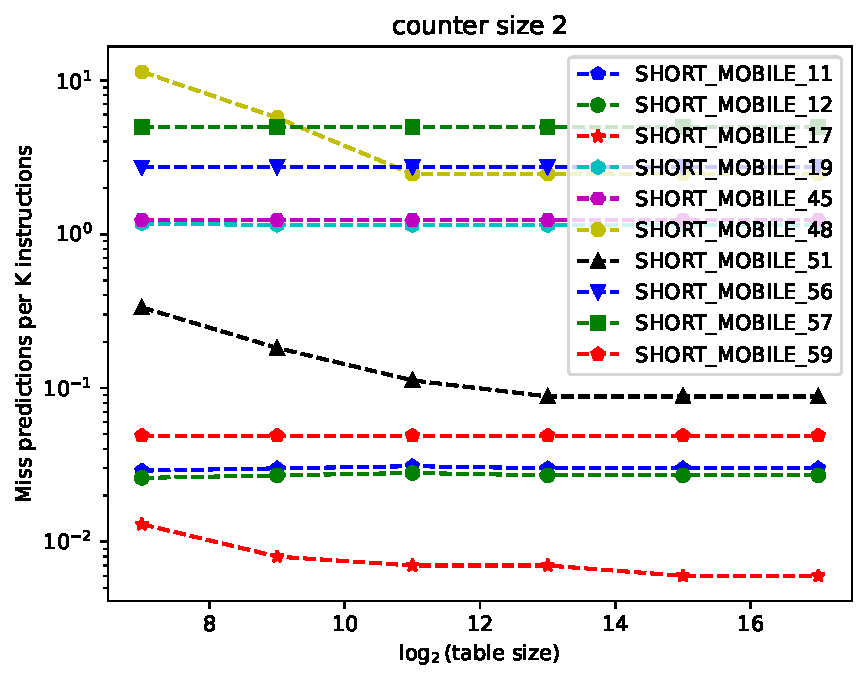
\includegraphics[width=.5\textwidth]{perceptron/h4/graph_2.pdf}
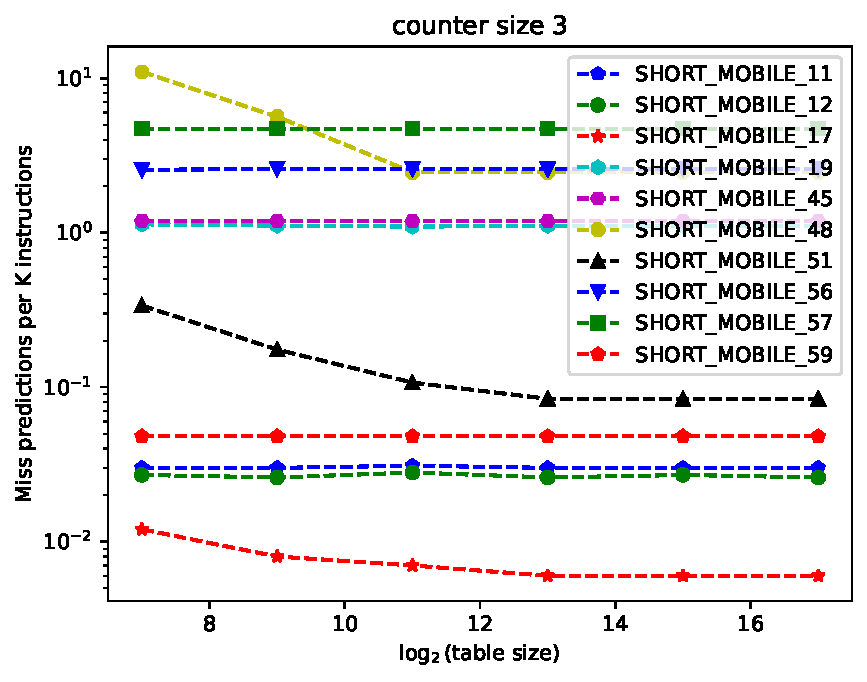
\includegraphics[width=.5\textwidth]{perceptron/h4/graph_3.pdf}
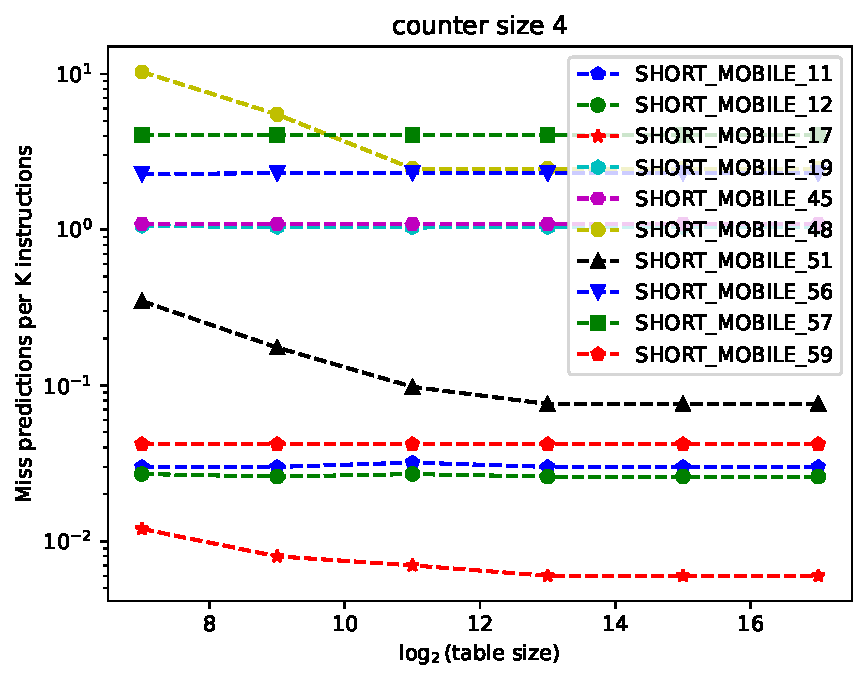
\includegraphics[width=.5\textwidth]{perceptron/h4/graph_4.pdf}

Pour le perceptron, le counter size tel qu'il était défini n'a pas beaucoup de sens. Nous avons donc décidé de l'utiliser pour tester plusieurs valeurs de theta. Dans les différents graphes, $theta = 2^{counter\_size}$.

Les valeurs obtenues avec le perceptron sont plutôt décevantes quand on considère un historique sur 4 bits. Les résultats pour les petites valeurs sont similaires au prédicteur gshare avec un historique sur 4 bits pour les petites tailles de table. Cependant, les résultats pour le prédicteur gshare sont meilleurs pour les grandes tailles de table que le perceptron.

\subsubsection{Historique sur 5 bits}

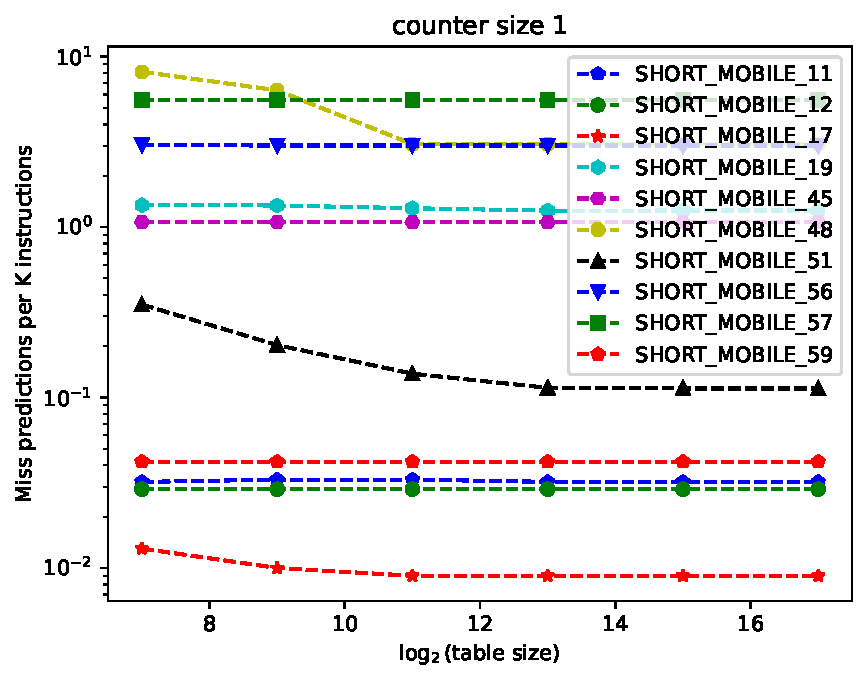
\includegraphics[width=.5\textwidth]{perceptron/h5/graph_1.pdf}
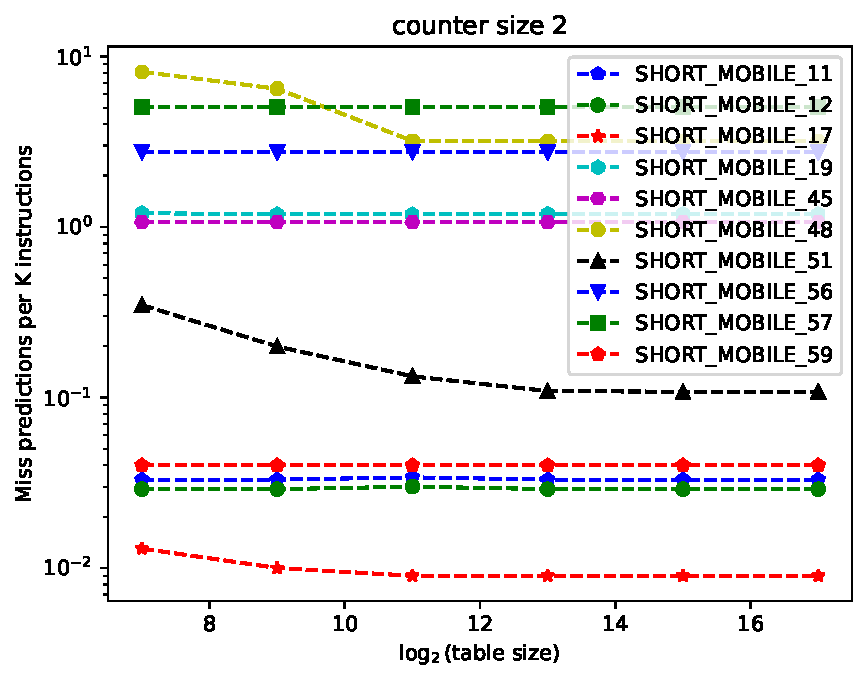
\includegraphics[width=.5\textwidth]{perceptron/h5/graph_2.pdf}
\includegraphics[width=.5\textwidth]{perceptron/h5/graph_3.pdf}
\includegraphics[width=.5\textwidth]{perceptron/h5/graph_4.pdf}

Les résultats de ce perceptron sont également décevants. Pour les petites tailles de table, ils sont parfois meilleurs que pour le perceptron avec historique sur 4 bits (remarquable notamment sur la courbe \textit{SHORT\_MOBILE\_48}. Cependant pour les grandes valeurs de table, ce perceptron est moins bon que le perceptron précédant. Cela se remarque notamment avec l'échantillon \textit{SHORT\_MOBILE\_17}.

\subsubsection{Historique sur 6 bits}

\includegraphics[width=.5\textwidth]{perceptron/h6/graph_1.pdf}
\includegraphics[width=.5\textwidth]{perceptron/h6/graph_2.pdf}
\includegraphics[width=.5\textwidth]{perceptron/h6/graph_3.pdf}
\includegraphics[width=.5\textwidth]{perceptron/h6/graph_4.pdf}

Ce perceptron est similaire aux perceptrons précédents. Cependant, l'échantillon \textit{SHORT\_MOBILE\_48} connaît moins d'erreurs de prédictions par instruction avec ce perceptron sur les petites valeurs.

Il reste toutefois décevant.

\subsubsection{Historique sur 59 bits}

\includegraphics[width=.5\textwidth]{perceptron/h59/graph_1.pdf}
\includegraphics[width=.5\textwidth]{perceptron/h59/graph_2.pdf}
\includegraphics[width=.5\textwidth]{perceptron/h59/graph_3.pdf}
\includegraphics[width=.5\textwidth]{perceptron/h59/graph_4.pdf}

Les résultats avec ce perceptron sont plus satisfaisant qu'avec les autres. Deux cas de figure se présentent :
\begin{itemize}
    \item Les résultats obtenus sont similaires à ceux du méta prédicteur. Par exemple, on peut considérer l'échantillon \textit{SHORT\_MOBILE\_45}.
    \item Les résultats obtenus sont meilleurs que ceux du méta prédicteur : \textit{SHORT\_MOBILE\_17}.
\end{itemize}
\newpage

\section{Conclusion}

Nous avons pu expérimenter plusieurs types de prédicteurs différents, se basant sur des techniques différentes. En premier lieux, nous pouvons faire une différence entre le prédicteur bimodal et les autres au travers du fait que seul le prédicteur bimodal n'utilise pas l'information d'historique. Au vu de la comparaison des résultats entre le bimodal et les autres prédicteurs, il semble que l'historique soit une information très pertinente en plus du PC quand il s'agit de prédire l'issue d'un branchement. Cela semble très cohérent dans les cas où on parcourt beaucoup de fois le même chemin dans l'arbre des branchements du programme.


Dans les prédicteurs à historique, le meilleur des prédicteurs considérés comme simple est le méta prédicteur, même s'il peut arriver que le prédicteur local soit légèrement meilleur sur certaines valeurs. C'est corrélé avec le fait que le prédicteur local est meilleur que le prédicteur à historique global dans une très large majorité de cas. Toutefois, cela vient avec un coût : la taille de la table à stocker en mémoire. En effet, avec un nombre de bits d'historique conséquent, la table d'historique local peut rapidement prendre beaucoup d'espace.

Le perceptron est quant à lui efficace si l'on prend les valeurs conseillées par le papier pour le nombre de bits d'historique. Il présente également l'avantage de ne pas avoir besoin de beaucoup de mémoire, étant donné que la taille de la table sur laquelle il travaille est en $n*nentries$, contrairement au prédicteur local dont la taille de table est en $2^{n}*nentries$, $n$ étant le nombre de bit d'historiques et $nentries = 2^{pcbits}$.

\end{document}
